\documentclass{standalone}
\usepackage{tikz} % tikz
\usepackage{standalone} % tikz figures are often in standalone
\usepackage{amsfonts} % mathbb etc
\usepackage{amsmath} % crucial package
\usepackage{amsthm} % ams-style theorems
\usepackage{bm} % bold math symbols
\usepackage{xcolor} % more colors
\usepackage[T1]{fontenc} % modern encoding, better than OT1, the default

\newtheorem{definition-fr}{Définition}
\newtheorem{example-fr}{Exemple}
\newtheorem{theorem-fr}{Théorème}
\newtheorem{proposition-fr}{Proposition}
\newtheorem{lemma-fr}{Lemme}
\newtheorem{remark-fr}{Remarque}
\newtheorem{definition}{Definition}
\newtheorem{lemma}{Lemma}
\newtheorem{proposition}{Proposition}
\newtheorem{remark}{Remark}

\usetikzlibrary{decorations.pathmorphing} % for snake, zigzag...
\usetikzlibrary{positioning} % for the "below of=1cm" type of options
\usetikzlibrary{intersections} % e.g. for pyramid
\usetikzlibrary{calc} % for computing node coordinates from others
\usetikzlibrary{overlay-beamer-styles} % when \pause glitches in tikz beamer
\usetikzlibrary{arrows} % arrows
\usetikzlibrary{external} % only compile the figure the first time
\tikzexternalize[only named=true, prefix=tikz-cache/]
\immediate\write18{mkdir -p latex-build/tikz-cache}

% used to pass "scale=XX" as includetikz option
\pgfkeys{
  /tikzoptions/.is family, % Namespace
  /tikzoptions/.cd, % Namespace
  scale/.store in=\scale, % Store the value of 'scale'
}

% usage: \includetikz[scale=XX]{fig}, fetches from my local database
\newcommand{\includetikz}[2][scale=1]{
  \bgroup
  \pgfkeys{/tikzoptions,#1} % currently only accepts 'scale' (april 9 2025)
  \tikzsetnextfilename{#2}
  \include{tex-macros/tikz-figures/#2}% Include the standalone TikZ file
  \egroup
}

% usage: \inputtikz[scale=XX]{fig}, fetches from my local database
\newcommand{\inputtikz}[2][scale=1]{
  \bgroup
  \pgfkeys{/tikzoptions,#1} % currently only accepts 'scale' (april 9 2025)
  \tikzsetnextfilename{#2}
  \input{tex-macros/tikz-figures/#2}% Include the standalone TikZ file
  \egroup
}


\newcommand{\bigOt}{\widetilde{\mathcal{O}}}
\newcommand{\bigO}{\mathcal{O}}

\definecolor{mypurp}{HTML}{8f0c97}
\definecolor{myred}{HTML}{9f103b}
\definecolor{myor}{HTML}{ae3011}
\definecolor{mydarkor1}{HTML}{96240f}
\definecolor{mydarkor2}{HTML}{7f180c}
\definecolor{mylb1}{HTML}{00557e}
\definecolor{mylb2}{HTML}{013157}
\definecolor{mybl1}{HTML}{0d08a9}
\definecolor{mybl2}{HTML}{04037f}
\definecolor{mygr1}{HTML}{097e3e}
\definecolor{mygr2}{HTML}{025520}
\definecolor{myyellow}{HTML}{FFD700}



\makeatletter
\@ifundefined{scale}{
  \def\scale{1}
}
\makeatother


\begin{document}
\begin{tikzpicture}
  \def\arrowlength{2em}
  \def\bigarrowlength{5em}
  \def\branchwidth{5em}
  \def\sboxw{2em}
  \def\sboxh{\sboxw}
  \def\linw{2em}

  \node (el1) at (0,0) {0};
  \node (el2) at (0, {-\branchwidth}) {$x_0$};

  \draw[->] (el1) --  ++(\arrowlength,0) coordinate (mup1);
  \draw[->] (mup1) ++(\linw,0) -- node[below] {$P_1(x_0)$} ++(\bigarrowlength,0) coordinate (sup1);
  \draw[->] (sup1) ++(\sboxw,0) --  ++(\arrowlength,0) coordinate (mup2);
  \draw[->] (mup2) ++(\linw,0) -- node[below] {$P_2(x_0,x_1)$} ++(\bigarrowlength,0) coordinate (sup2);
  \draw[->] (sup2) ++(\sboxw,0) --  ++(\arrowlength,0) coordinate (mup3);
  \draw[->] (mup3) ++(\linw,0) -- ++(\arrowlength,0) node[anchor=west] (endup) {$G(x_0, x_1, x_2)$};

  \draw[->] (el2) --  ++(\arrowlength,0) coordinate (mdown1);
  \draw[->] (mdown1) ++(\linw,0) -- node[above] {$Q_1(x_0)$} ++(\bigarrowlength,0) coordinate (sdown1);
  \draw[->] (sdown1) ++(\sboxw,0) --node[above] {$x_1$} ++(\arrowlength,0) coordinate (mdown2);
  \draw[->] (mdown2) ++(\linw,0) -- node[above] {$Q_2(x_0,x_1)$} ++(\bigarrowlength,0) coordinate (sdown2);
  \draw[->] (sdown2) ++(\sboxw,0) -- node[above] {$x_2$} ++(\arrowlength,0) coordinate (mdown3);
  \draw[->] (mdown3) ++(\linw,0) -- ++(\arrowlength,0) node[anchor=west] (enddown) {$\ast$};

  \foreach \i in {1,2} {
    \draw[rounded corners]
    ($(sup\i) + (0,-0.5*\sboxh)$) rectangle node {$x^\alpha$}
    ($(sup\i) + (\sboxw,0.5*\sboxh)$);

    \draw[rounded corners]
    ($(sdown\i) + (0,-0.5*\sboxh)$) rectangle node {$x^{\sfrac{1}{\alpha}}$}
    ($(sdown\i) + (\sboxw,0.5*\sboxh)$);
  }

  \foreach \i in {1,2,3} {
    \coordinate (mcorner1) at ($(mup\i) + (0, 0.5*\sboxh)$);
    \coordinate (mcorner2) at ($(mdown\i) + (\linw, -0.5*\sboxh)$);
    \draw[rounded corners] (mcorner1) rectangle node {$A$} (mcorner2);
  }

\end{tikzpicture}
\end{document}
